% !TEX TS-program = pdflatex
\documentclass[11pt]{article}

% -------------------- Packages --------------------
\usepackage[a4paper,margin=1in]{geometry}
\usepackage{amsmath,amssymb}
\usepackage[T1]{fontenc}
\usepackage{lmodern}
\usepackage{xcolor}
\usepackage{tcolorbox}
\tcbuselibrary{skins,breakable}
\usepackage{enumitem}
\usepackage{hyperref}
\usepackage{tikz}
\usetikzlibrary{calc,angles,quotes,arrows.meta,intersections}

\pagestyle{empty}

% -------------------- Dark Theme Colors --------------------
\definecolor{bg}{HTML}{000000}
\definecolor{pairbg}{HTML}{121212}
\definecolor{solbg}{HTML}{0A0A0A}
\definecolor{border}{HTML}{2A2A2A}
\definecolor{text}{HTML}{FFFFFF}
\definecolor{muted}{HTML}{C9CDD3}
\definecolor{gold}{HTML}{FFD700}
\definecolor{green}{HTML}{4ADE80}
\definecolor{cyan}{HTML}{38BDF8}

\pagecolor{bg}
\color{text}

\hypersetup{
  colorlinks=true,
  linkcolor=cyan,
  urlcolor=cyan
}

\setlength{\parindent}{0pt}
\setlength{\parskip}{10pt}

\setlist[itemize]{left=1.4em,itemsep=6pt,topsep=6pt}
\setlist[enumerate]{left=1.6em,itemsep=4pt,topsep=4pt}

% -------------------- tcolorbox Base --------------------
\tcbset{
  enhanced,
  breakable,
  arc=12pt,
  boxrule=0.8pt,
  left=16pt,right=16pt,top=12pt,bottom=12pt
}

\newtcolorbox{QAPair}[1]{%
  colback=pairbg,
  colbacklower=solbg,
  colframe=border,
  coltext=text,
  title=\textcolor{gold}{\bfseries #1},
  fonttitle=\bfseries,
  coltitle=text,
  segmentation style={draw=border, dashed, line width=0.6pt},
}

\newtcolorbox{QuickBox}{%
  colback=pairbg,
  colframe=cyan,
  coltext=text,
  fontupper=\color{text},
  borderline north={4pt}{0pt}{cyan},
  arc=14pt,
  boxrule=0.8pt
}

\newtcolorbox{ConceptBox}[1]{%
  colback=solbg,
  colframe=border,
  coltext=text,
  arc=14pt,
  boxrule=0.8pt,
  left=14pt,right=14pt,top=10pt,bottom=10pt,
  breakable,
  title=\textcolor{gold}{\bfseries #1},
  fonttitle=\bfseries,
  coltitle=text,
}

\newcommand{\Step}[1]{\textcolor{muted}{\textbf{Step #1:}}}

% TikZ defaults for dark background
\tikzset{
  line/.style={draw=text, line width=0.95pt},
  dashedline/.style={draw=muted, line width=0.85pt, dashed},
  cline/.style={draw=cyan, line width=1.05pt},
  gline/.style={draw=green, line width=1.05pt},
  dot/.style={circle, fill=text, inner sep=1.35pt},
  lbl/.style={text=text, font=\small},
  mlabel/.style={text=muted, font=\small}
}

\newcommand{\FigTitle}[1]{\textcolor{muted}{\textbf{#1}}\par\medskip}

\newcommand{\StepFig}[2]{%
\begin{center}
\FigTitle{#1}
#2
\end{center}
}

% ============================================================
% QUICK-FORMULA DIAGRAM MACROS (one diagram per concept)
% ============================================================

% (QF1) Perpendicular from centre to chord bisects chord
\newcommand{\QFDiagPerpBisect}{%
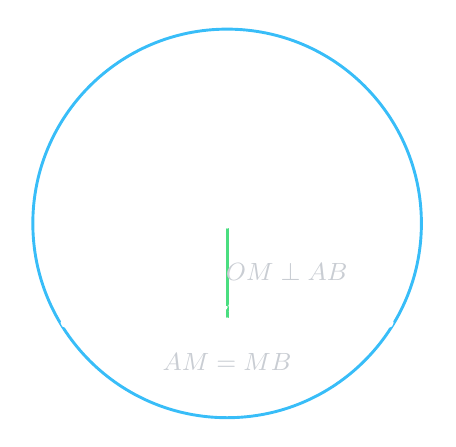
\begin{tikzpicture}[scale=1.05]
  \coordinate (O) at (0,0.65);
  \def\r{2.35}
  \draw[cline] (O) circle (\r);

  \coordinate (A) at (-1.95,-0.55);
  \coordinate (B) at ( 1.95,-0.55);
  \coordinate (M) at ($(A)!0.5!(B)$);

  \draw[line] (A)--(B);
  \draw[gline] (O)--(M);

  % right angle at M
  \draw[line] ($(M)+(-0.18,0)$) -- ($(M)+(-0.18,0.18)$) -- ($(M)+(0,0.18)$);

  \fill (O) node[dot]{} node[lbl, above right] {$O$};
  \fill (A) node[dot]{} node[lbl, below left] {$A$};
  \fill (B) node[dot]{} node[lbl, below right] {$B$};
  \fill (M) node[dot]{} node[lbl, above] {$M$};

  \node[mlabel] at (0,-1.02) {$AM=MB$};
  \node[mlabel] at (0.72,0.07) {$OM\perp AB$};
\end{tikzpicture}
}

% (QF2) Chord length = 2*sqrt(r^2-d^2)
\newcommand{\QFDiagChordLength}{%
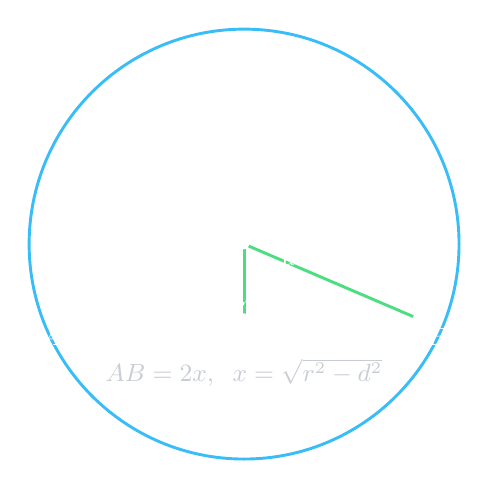
\begin{tikzpicture}[scale=1.05]
  \coordinate (O) at (0,0);
  \def\r{2.6}
  \draw[cline] (O) circle (\r);

  % chord endpoints (horizontal)
  \coordinate (A) at (-2.1,-0.9);
  \coordinate (B) at ( 2.1,-0.9);
  \coordinate (M) at ($(A)!0.5!(B)$);

  \draw[line] (A)--(B);
  \draw[gline] (O)--(M);
  \draw[gline] (O)--(B);

  % right angle marker at M
  \draw[line] ($(M)+(-0.18,0)$) -- ($(M)+(-0.18,0.18)$) -- ($(M)+(0,0.18)$);

  \fill (O) node[dot]{} node[lbl, above left] {$O$};
  \fill (A) node[dot]{} node[lbl, below left] {$A$};
  \fill (B) node[dot]{} node[lbl, below right] {$B$};
  \fill (M) node[dot]{} node[lbl, above] {$M$};

  \node[lbl] at (1.05,0.35) {$r$};
  \node[lbl] at (0.55,-0.15) {$d$};
  \node[lbl] at (1.25,-1.20) {$x$};

  \node[mlabel] at (0,-1.55) {$AB=2x,\;\; x=\sqrt{r^2-d^2}$};
\end{tikzpicture}
}

% (QF3) Equilateral triangle circumradius
\newcommand{\QFDiagEquilateral}{%
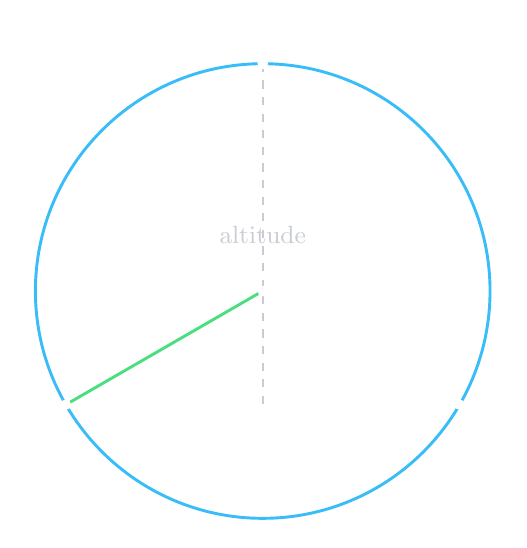
\begin{tikzpicture}[scale=1.0]
  % Equilateral with side a=5 units
  \coordinate (A) at (0,0);
  \coordinate (B) at (5,0);
  \coordinate (C) at (2.5,4.330);
  \coordinate (O) at (2.5,1.443); % circumcenter/centroid

  \draw[line] (A)--(B)--(C)--cycle;
  \draw[cline] (O) circle (2.887);

  \draw[gline] (O)--(A);
  \draw[dashedline] (C)--(2.5,0); % altitude

  \fill (A) node[dot]{} node[lbl, below left] {$A$};
  \fill (B) node[dot]{} node[lbl, below right] {$B$};
  \fill (C) node[dot]{} node[lbl, above] {$C$};
  \fill (O) node[dot]{} node[lbl, right] {$O$};

  \node[lbl] at (2.5,-0.55) {$a$};
  \node[lbl] at (3.25,0.95) {$R$};
  \node[mlabel] at (2.5,2.15) {altitude};
\end{tikzpicture}
}

% (QF4) Rectangle circumcircle (diagonals meet at centre)
\newcommand{\QFDiagRectangle}{%
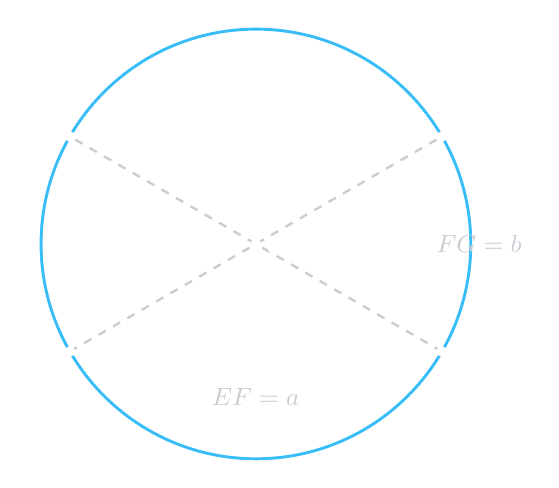
\begin{tikzpicture}[scale=1.05]
  \coordinate (E) at (0,0);
  \coordinate (F) at (4.5,0);
  \coordinate (G) at (4.5,2.6);
  \coordinate (H) at (0,2.6);
  \coordinate (O) at ($(E)!0.5!(G)$);

  \draw[line] (E)--(F)--(G)--(H)--cycle;
  \draw[dashedline] (E)--(G);
  \draw[dashedline] (F)--(H);
  \draw[cline] (O) circle ({0.5*sqrt((4.5)^2 + (2.6)^2)});

  \fill (E) node[dot]{} node[lbl, below left] {$E$};
  \fill (F) node[dot]{} node[lbl, below right] {$F$};
  \fill (G) node[dot]{} node[lbl, above right] {$G$};
  \fill (H) node[dot]{} node[lbl, above left] {$H$};
  \fill (O) node[dot]{} node[lbl, right] {$O$};

  \node[mlabel] at (2.25,-0.55) {$EF=a$};
  \node[mlabel] at (4.95,1.3) {$FG=b$};
\end{tikzpicture}
}

% (QF5) Distance formula diagram on coordinate plane
\newcommand{\QFDiagDistance}{%
\begin{tikzpicture}[scale=1.0]
  % axes
  \draw[dashedline, -{Stealth[length=3mm]}] (-0.2,0) -- (5.2,0) node[lbl, right] {$x$};
  \draw[dashedline, -{Stealth[length=3mm]}] (0,-0.2) -- (0,4.2) node[lbl, above] {$y$};

  \coordinate (O) at (1,1);
  \coordinate (C) at (4,3.2);

  \draw[gline] (O)--(C);

  % projections (dx, dy)
  \draw[dashedline] (O) -- (4,1);
  \draw[dashedline] (4,1) -- (C);

  \fill (O) node[dot]{} node[lbl, below left] {$(x_1,y_1)$};
  \fill (C) node[dot]{} node[lbl, above right] {$(x_2,y_2)$};

  \node[mlabel] at (2.5,0.72) {$\Delta x$};
  \node[mlabel] at (4.35,2.1) {$\Delta y$};
  \node[lbl] at (2.8,2.35) {$OC$};
\end{tikzpicture}
}

% ============================================================
% SMALL STEP DIAGRAM MACROS (reused)
% ============================================================

% Generic circle with centre P, chord AB, perpendicular PD
\newcommand{\DiagCentrePerpChord}{%
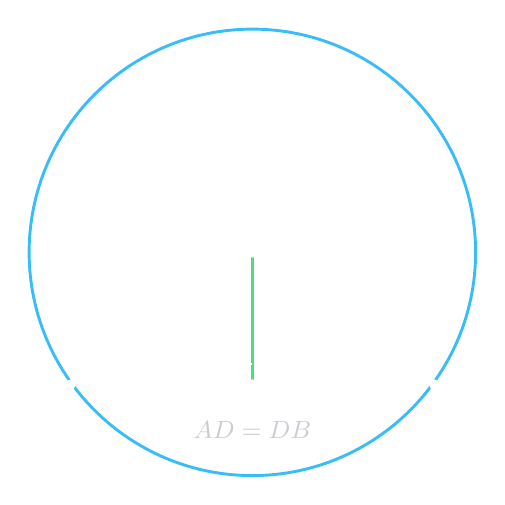
\begin{tikzpicture}[scale=1.05]
  \coordinate (P) at (0,1.6);
  \coordinate (D) at (0,0);
  \coordinate (A) at (-2.2,0);
  \coordinate (B) at (2.2,0);

  \draw[cline] (P) circle (2.7);
  \draw[line] (A)--(B);
  \draw[gline] (P)--(D);

  % right angle at D
  \draw[line] (-0.25,0) -- (-0.25,0.25) -- (0,0.25);

  \fill (P) node[dot]{} node[lbl, right] {$P$};
  \fill (D) node[dot]{} node[lbl, below] {$D$};
  \fill (A) node[dot]{} node[lbl, below left] {$A$};
  \fill (B) node[dot]{} node[lbl, below right] {$B$};

  \node[mlabel] at (0,-0.55) {$AD=DB$};
\end{tikzpicture}
}

% Right triangle PDB (focus)
\newcommand{\DiagRightTrianglePDB}{%
\begin{tikzpicture}[scale=1.05]
  \coordinate (D) at (0,0);
  \coordinate (B) at (2.6,0);
  \coordinate (P) at (0,2.0);

  \draw[line] (D)--(B)--(P)--cycle;
  \draw[line] (-0.25,0) -- (-0.25,0.25) -- (0,0.25);

  \fill (P) node[dot]{} node[lbl, left] {$P$};
  \fill (D) node[dot]{} node[lbl, below] {$D$};
  \fill (B) node[dot]{} node[lbl, below right] {$B$};

  \node[lbl] at (1.45,1.25) {$PB$};
  \node[lbl] at (0.55,1.1) {$PD$};
  \node[lbl] at (1.3,-0.35) {$DB$};
\end{tikzpicture}
}

% Circle + chord AB with midpoint E and radius computed
\newcommand{\DiagChordWithMidpointE}{%
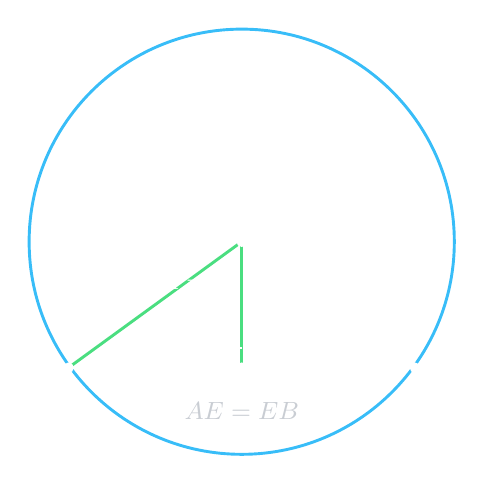
\begin{tikzpicture}[scale=1.0]
  \coordinate (P) at (0,1.6);
  \coordinate (E) at (0,0);
  \coordinate (A) at (-2.2,0);
  \coordinate (B) at (2.2,0);

  \draw[cline] (P) circle (2.7);
  \draw[line] (A)--(B);
  \draw[gline] (P)--(E);
  \draw[gline] (P)--(A);

  \draw[line] (-0.25,0) -- (-0.25,0.25) -- (0,0.25);

  \fill (P) node[dot]{} node[lbl, right] {$P$};
  \fill (E) node[dot]{} node[lbl, below] {$E$};
  \fill (A) node[dot]{} node[lbl, below left] {$A$};
  \fill (B) node[dot]{} node[lbl, below right] {$B$};

  \node[mlabel] at (0,-0.55) {$AE=EB$};
  \node[lbl] at (0.65,0.65) {$PE$};
  \node[lbl] at (-0.75,1.1) {$PA=r$};
\end{tikzpicture}
}

% ============================================================
\begin{document}

\begin{center}
{\LARGE\bfseries \textcolor{gold}{Exercise 9.1 --- Solutions}}\\[-2pt]
\end{center}

% ============================================================
% QUICK FORMULAS: EACH CONCEPT + ITS OWN DIAGRAM (no overflow)
\begin{QuickBox}
{\color{cyan}\bfseries Quick formulas / facts}\par\medskip

\begin{ConceptBox}{1) Perpendicular from centre to a chord bisects the chord}
\[
\text{If } OM\perp AB \text{ and } O \text{ is centre, then } AM=MB.
\]
\StepFig{Diagram for the fact}{\QFDiagPerpBisect}
\end{ConceptBox}

\begin{ConceptBox}{2) Chord-length formula}
If radius is $r$ and distance from centre to chord is $d$, then
\[
\text{Chord length }=2\sqrt{r^2-d^2}.
\]
\StepFig{Diagram (half-chord $x=\sqrt{r^2-d^2}$)}{\QFDiagChordLength}
\end{ConceptBox}

\begin{ConceptBox}{3) Equilateral triangle (side $a$)}
\[
\text{Altitude }=\frac{\sqrt3}{2}a,\qquad
R=\frac{a}{\sqrt3}=\frac{a\sqrt3}{3}.
\]
\StepFig{Diagram (equilateral $\triangle ABC$ and circumradius $R$)}{\QFDiagEquilateral}
\end{ConceptBox}

\begin{ConceptBox}{4) Rectangle $a\times b$ (circumcircle)}
Circumcentre is intersection of diagonals; radius is half the diagonal:
\[
R=\frac12\sqrt{a^2+b^2}.
\]
\StepFig{Diagram (rectangle + diagonals + circumcircle)}{\QFDiagRectangle}
\end{ConceptBox}

\begin{ConceptBox}{5) Distance formula (coordinates)}
\[
OC=\sqrt{(x_2-x_1)^2+(y_2-y_1)^2}.
\]
\StepFig{Diagram (showing $\Delta x$ and $\Delta y$)}{\QFDiagDistance}
\end{ConceptBox}

\end{QuickBox}

% ============================================================
% Q1
\begin{QAPair}{Question 1}
\textcolor{gold}{\bfseries Question:}
Construct an equilateral triangle with side $5$ cm long. Show that one and only one circle can be drawn through the vertices of the triangle.
What is the radius of the circle drawn?\\
\tcblower
\textcolor{green}{\bfseries Answer:}

\Step{1 (Construction of $\triangle ABC$).}
\begin{enumerate}
\item Draw the line segment $AB=5$ cm.
\item With centre $A$ and radius $AB$, draw an arc above $AB$.
\item With centre $B$ and radius $AB$, draw another arc intersecting the first arc at $C$.
\item Join $AC$ and $BC$. Then $\triangle ABC$ is equilateral.
\end{enumerate}

\StepFig{Step 1(a): Draw $AB=5$ cm}{%
\begin{tikzpicture}[scale=1.0]
  \coordinate (A) at (0,0);
  \coordinate (B) at (5,0);
  \draw[line] (A)--(B);
  \fill (A) node[dot]{} node[lbl, below left]{$A$};
  \fill (B) node[dot]{} node[lbl, below right]{$B$};
  \node[lbl] at (2.5,-0.55) {$5\text{ cm}$};
\end{tikzpicture}
}

\StepFig{Step 1(b--c): Draw arcs; mark intersection $C$}{%
\begin{tikzpicture}[scale=0.95]
  \coordinate (A) at (0,0);
  \coordinate (B) at (5,0);
  \coordinate (C) at (2.5,4.330);

  \draw[line] (A)--(B);
  \def\r{5}
  \draw[cline] (A) ++(10:\r) arc (10:170:\r);
  \draw[cline] (B) ++(170:\r) arc (170:10:\r);

  \fill (A) node[dot]{} node[lbl, below left]{$A$};
  \fill (B) node[dot]{} node[lbl, below right]{$B$};
  \fill (C) node[dot]{} node[lbl, above]{$C$};
  \node[mlabel] at (2.5,2.75) {arcs intersect at $C$};
\end{tikzpicture}
}

\StepFig{Step 1(d): Join $AC$ and $BC$}{%
\begin{tikzpicture}[scale=0.95]
  \coordinate (A) at (0,0);
  \coordinate (B) at (5,0);
  \coordinate (C) at (2.5,4.330);
  \draw[line] (A)--(B)--(C)--cycle;
  \fill (A) node[dot]{} node[lbl, below left]{$A$};
  \fill (B) node[dot]{} node[lbl, below right]{$B$};
  \fill (C) node[dot]{} node[lbl, above]{$C$};
  \node[mlabel] at (2.5,-0.55) {$AB=BC=CA$};
\end{tikzpicture}
}

\Step{2 (Show the circle is unique).}
Draw perpendicular bisectors of two sides (e.g.\ $AB$ and $BC$).  
They intersect at exactly one point $O$ (circumcentre).  
Then $OA=OB=OC$, so the circle with centre $O$ and radius $OA$ passes through $A,B,C$.  
A circle through three non-collinear points is unique.

\StepFig{Step 2: Perpendicular bisectors meet at a single point $O$}{%
\begin{tikzpicture}[scale=0.95]
  \coordinate (A) at (0,0);
  \coordinate (B) at (5,0);
  \coordinate (C) at (2.5,4.330);
  \coordinate (Mab) at ($(A)!0.5!(B)$);
  \coordinate (Mbc) at ($(B)!0.5!(C)$);
  \coordinate (O) at (2.5,1.443);

  \draw[line] (A)--(B)--(C)--cycle;

  \draw[dashedline] (Mab) ++(0,-1.2) -- ++(0,3.2);            % perp bisector of AB
  \draw[dashedline] (Mbc) ++(-2.6,-1.45) -- ++(5.2,2.9);      % perp bisector of BC

  \fill (O) node[dot]{} node[lbl, right]{$O$};
  \fill (A) node[dot]{} node[lbl, below left]{$A$};
  \fill (B) node[dot]{} node[lbl, below right]{$B$};
  \fill (C) node[dot]{} node[lbl, above]{$C$};
\end{tikzpicture}
}

\Step{3 (Draw the circumcircle).}
With centre $O$ and radius $OA$, draw the circle.

\StepFig{Step 3: Circle through $A,B,C$}{%
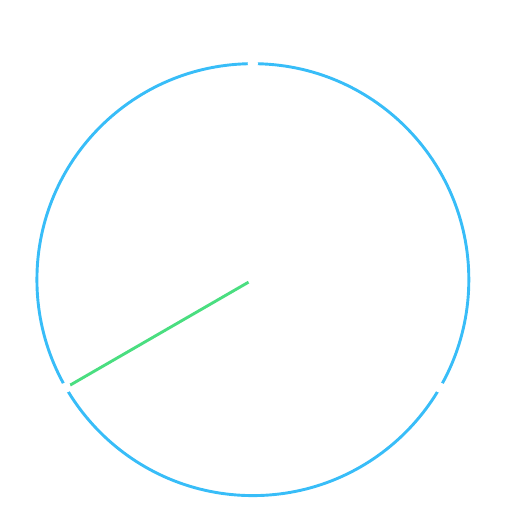
\begin{tikzpicture}[scale=0.95]
  \coordinate (A) at (0,0);
  \coordinate (B) at (5,0);
  \coordinate (C) at (2.5,4.330);
  \coordinate (O) at (2.5,1.443);
  \def\R{2.887}

  \draw[cline] (O) circle (\R);
  \draw[line] (A)--(B)--(C)--cycle;
  \draw[gline] (O)--(A);

  \fill (O) node[dot]{} node[lbl, right]{$O$};
  \fill (A) node[dot]{} node[lbl, below left]{$A$};
  \fill (B) node[dot]{} node[lbl, below right]{$B$};
  \fill (C) node[dot]{} node[lbl, above]{$C$};

  \node[lbl] at (3.25,0.95) {$R=OA$};
\end{tikzpicture}
}

\Step{4 (Radius).}
For side $a$ of an equilateral triangle:
\[
R=\frac{a}{\sqrt3}.
\]
So for $a=5$ cm:
\[
R=\frac{5}{\sqrt3}=\frac{5\sqrt3}{3}\ \text{cm}.
\]

\StepFig{Step 4: Formula-map for equilateral triangle}{\QFDiagEquilateral}
\end{QAPair}

% ============================================================
% Q2(i)
\begin{QAPair}{Question 2 (i)}
\textcolor{gold}{\bfseries Question:}
Given $P$ is the centre and $PD\perp AB$. If $PA=5$ cm and $PD=3$ cm, find $x=DB$.\\
\tcblower
\textcolor{green}{\bfseries Answer:}

\Step{1.} $PD\perp AB$ with centre $P$ $\Rightarrow$ $D$ bisects chord $AB$:
\[
AD=DB=x.
\]
\StepFig{Step 1 diagram (centre $\perp$ chord)}{\DiagCentrePerpChord}

\Step{2.} In right $\triangle PDB$:
\[
PB^2=PD^2+DB^2.
\]
Since $PB=PA=5$:
\[
5^2=3^2+x^2 \Rightarrow 25=9+x^2 \Rightarrow x^2=16 \Rightarrow x=4\text{ cm}.
\]
\StepFig{Step 2 diagram (right triangle used)}{\DiagRightTrianglePDB}
\end{QAPair}

% ============================================================
% Q2(ii)
\begin{QAPair}{Question 2 (ii)}
\textcolor{gold}{\bfseries Question:}
Given $P$ is the centre and $PD\perp EF$. If $PF=10$ cm and $DF=8$ cm, find $y=PD$.\\
\tcblower
\textcolor{green}{\bfseries Answer:}

\Step{1.} $PD\perp EF$ with centre $P$ $\Rightarrow$ $D$ bisects chord $EF$:
\[
DE=DF=8\text{ cm}.
\]
\StepFig{Step 1 diagram (bisected chord)}{%
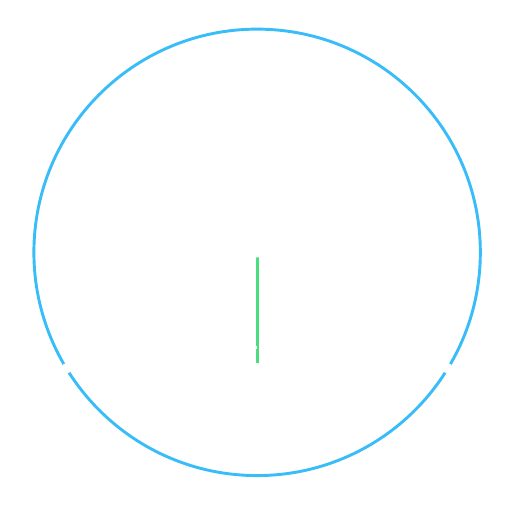
\begin{tikzpicture}[scale=1.05]
  \coordinate (P) at (0,1.4);
  \coordinate (D) at (0,0);
  \coordinate (E) at (-2.3,0);
  \coordinate (F) at (2.3,0);

  \draw[cline] (P) circle (2.7);
  \draw[line] (E)--(F);
  \draw[gline] (P)--(D);
  \draw[line] (-0.25,0) -- (-0.25,0.25) -- (0,0.25);

  \fill (P) node[dot]{} node[lbl, above] {$P$};
  \fill (D) node[dot]{} node[lbl, below] {$D$};
  \fill (E) node[dot]{} node[lbl, below left] {$E$};
  \fill (F) node[dot]{} node[lbl, below right] {$F$};

  \node[lbl] at (1.15,-0.35) {$8$};
  \node[lbl] at (-1.15,-0.35) {$8$};
\end{tikzpicture}
}

\Step{2.} In right $\triangle PDF$:
\[
PF^2=PD^2+DF^2
\Rightarrow 10^2=y^2+8^2
\Rightarrow y^2=36
\Rightarrow y=6\text{ cm}.
\]
\StepFig{Step 2 diagram (right triangle used)}{%
\begin{tikzpicture}[scale=1.05]
  \coordinate (D) at (0,0);
  \coordinate (F) at (2.6,0);
  \coordinate (P) at (0,2.0);

  \draw[line] (D)--(F)--(P)--cycle;
  \draw[line] (-0.25,0) -- (-0.25,0.25) -- (0,0.25);

  \fill (P) node[dot]{} node[lbl, left] {$P$};
  \fill (D) node[dot]{} node[lbl, below] {$D$};
  \fill (F) node[dot]{} node[lbl, below right] {$F$};

  \node[lbl] at (1.45,1.25) {$PF=10$};
  \node[lbl] at (0.65,1.1) {$PD=y$};
  \node[lbl] at (1.3,-0.35) {$DF=8$};
\end{tikzpicture}
}
\end{QAPair}

% ============================================================
% Q3
\begin{QAPair}{Question 3}
\textcolor{gold}{\bfseries Question:}
Find the length of diameter $CD$ of the circle when $AB=10$ cm and $PE=12$ cm. Also find $CE$.\\
\tcblower
\textcolor{green}{\bfseries Answer:}

\Step{1.} Centre-perpendicular to chord bisects the chord:
\[
AE=EB=\frac{AB}{2}=\frac{10}{2}=5\text{ cm}.
\]
\StepFig{Step 1 diagram (midpoint of chord)}{\DiagChordWithMidpointE}

\Step{2.} In right $\triangle PEA$:
\[
PA^2=PE^2+AE^2
\Rightarrow r^2=12^2+5^2=169
\Rightarrow r=13\text{ cm}.
\]
\StepFig{Step 2 diagram (right triangle $PEA$)}{%
\begin{tikzpicture}[scale=1.05]
  \coordinate (E) at (0,0);
  \coordinate (A) at (-2.6,0);
  \coordinate (P) at (0,2.0);

  \draw[line] (A)--(E)--(P)--cycle;
  \draw[line] (-0.25,0) -- (-0.25,0.25) -- (0,0.25);

  \fill (P) node[dot]{} node[lbl, right] {$P$};
  \fill (E) node[dot]{} node[lbl, below] {$E$};
  \fill (A) node[dot]{} node[lbl, below left] {$A$};

  \node[lbl] at (-1.3,-0.35) {$AE=5$};
  \node[lbl] at (0.55,1.1) {$PE=12$};
  \node[lbl] at (-1.25,1.15) {$PA=r$};
\end{tikzpicture}
}

\Step{3.} Diameter:
\[
CD=2r=2(13)=26\text{ cm}.
\]
\StepFig{Step 3 diagram (diameter = $2r$)}{%
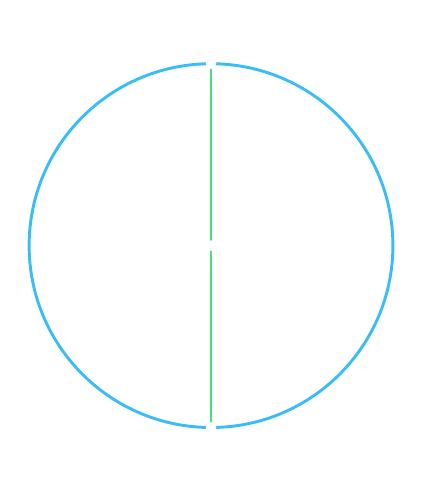
\begin{tikzpicture}[scale=1.05]
  \coordinate (P) at (0,0);
  \def\r{2.2}
  \draw[cline] (P) circle (\r);

  \coordinate (C) at (0,\r);
  \coordinate (D) at (0,-\r);
  \draw[gline] (C)--(D);

  \fill (P) node[dot]{} node[lbl, right] {$P$};
  \fill (C) node[dot]{} node[lbl, above] {$C$};
  \fill (D) node[dot]{} node[lbl, below] {$D$};

  \node[lbl] at (0.65,0) {$CD=2r$};
\end{tikzpicture}
}

\Step{4.} Since $PC=r=13$ and $PE=12$:
\[
CE=PC-PE=13-12=1\text{ cm}.
\]
\StepFig{Step 4 diagram ($CE$ is the difference along the radius)}{%
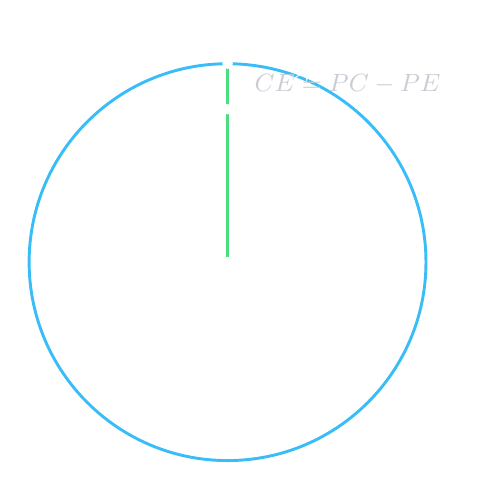
\begin{tikzpicture}[scale=1.05]
  \coordinate (P) at (0,0);
  \def\r{2.4}
  \draw[cline] (P) circle (\r);

  \coordinate (C) at (0,\r);
  \coordinate (E) at (0,1.85);

  \draw[gline] (P)--(C);
  \draw[gline] (P)--(E);

  \fill (P) node[dot]{} node[lbl, right] {$P$};
  \fill (C) node[dot]{} node[lbl, above] {$C$};
  \fill (E) node[dot]{} node[lbl, right] {$E$};

  \node[lbl] at (0.75,1.2) {$PE$};
  \node[lbl] at (0.75,2.15) {$PC$};
  \node[mlabel] at (1.45,2.15) {$CE=PC-PE$};
\end{tikzpicture}
}
\end{QAPair}

% ============================================================
% Q4
\begin{QAPair}{Question 4}
\textcolor{gold}{\bfseries Question:}
In the diagram, $OB=15$ cm and $OF=9$ cm. Find the length of chord $CD$ given that $OF\perp CD$.\\
\tcblower
\textcolor{green}{\bfseries Answer:}

\Step{1.} $OF\perp CD$ $\Rightarrow$ $F$ bisects chord $CD$:
\[
CF=FD.
\]
\StepFig{Step 1 diagram (bisected chord)}{%
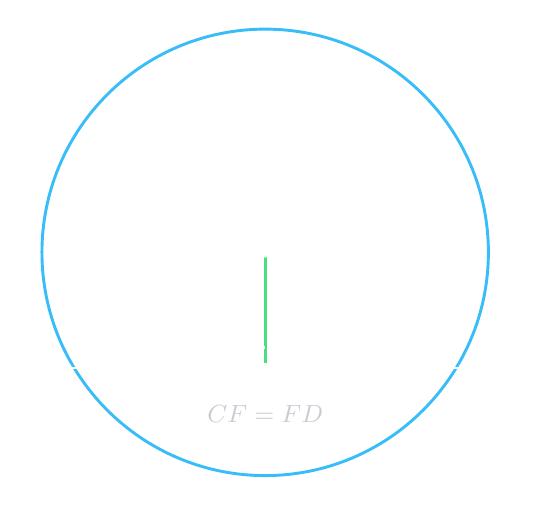
\begin{tikzpicture}[scale=1.05]
  \coordinate (O) at (0,1.4);
  \coordinate (F) at (0,0);
  \coordinate (C) at (-2.4,0);
  \coordinate (D) at (2.4,0);

  \draw[cline] (O) circle (2.7);
  \draw[line] (C)--(D);
  \draw[gline] (O)--(F);
  \draw[line] (-0.25,0) -- (-0.25,0.25) -- (0,0.25);

  \fill (O) node[dot]{} node[lbl, above] {$O$};
  \fill (F) node[dot]{} node[lbl, below] {$F$};
  \fill (C) node[dot]{} node[lbl, below left] {$C$};
  \fill (D) node[dot]{} node[lbl, below right] {$D$};

  \node[mlabel] at (0,-0.55) {$CF=FD$};
\end{tikzpicture}
}

\Step{2.} In right $\triangle OFD$:
\[
OD^2=OF^2+FD^2.
\]
With $OD=OB=15$ and $OF=9$:
\[
15^2=9^2+FD^2 \Rightarrow FD^2=144 \Rightarrow FD=12\text{ cm}.
\]
\StepFig{Step 2 diagram (right triangle used)}{%
\begin{tikzpicture}[scale=1.05]
  \coordinate (F) at (0,0);
  \coordinate (D) at (2.7,0);
  \coordinate (O) at (0,2.1);

  \draw[line] (O)--(F)--(D)--cycle;
  \draw[line] (-0.25,0) -- (-0.25,0.25) -- (0,0.25);

  \fill (O) node[dot]{} node[lbl, left] {$O$};
  \fill (F) node[dot]{} node[lbl, below] {$F$};
  \fill (D) node[dot]{} node[lbl, below right] {$D$};

  \node[lbl] at (1.45,1.25) {$OD=15$};
  \node[lbl] at (0.65,1.1) {$OF=9$};
  \node[lbl] at (1.35,-0.35) {$FD$};
\end{tikzpicture}
}

\Step{3.} Hence:
\[
CD=2FD=2(12)=24\text{ cm}.
\]
\StepFig{Step 3 diagram (full chord)}{%
\begin{tikzpicture}[scale=1.05]
  \coordinate (F) at (0,0);
  \coordinate (C) at (-2.7,0);
  \coordinate (D) at (2.7,0);

  \draw[line] (C)--(D);
  \fill (F) node[dot]{} node[lbl, below] {$F$};
  \fill (C) node[dot]{} node[lbl, below left] {$C$};
  \fill (D) node[dot]{} node[lbl, below right] {$D$};

  \node[lbl] at (-1.35,-0.35) {$12$};
  \node[lbl] at (1.35,-0.35) {$12$};
  \node[mlabel] at (0,-0.85) {$CD=24$};
\end{tikzpicture}
}
\end{QAPair}

% ============================================================
% Q5
\begin{QAPair}{Question 5}
\textcolor{gold}{\bfseries Question:}
Calculate the length of chord $AB$ if $OC\perp AB$. Given $OA=13$ cm, $O(3,6)$ and $C(7,9)$.\\
\tcblower
\textcolor{green}{\bfseries Answer:}

\Step{1.} Distance:
\[
OC=\sqrt{(7-3)^2+(9-6)^2}=\sqrt{4^2+3^2}=5\text{ cm}.
\]
\StepFig{Step 1 diagram (coordinates and $OC$)}{\QFDiagDistance}

\Step{2.} $OC\perp AB$ $\Rightarrow$ $C$ bisects chord $AB$:
\[
AC=CB=\frac{AB}{2}.
\]
\StepFig{Step 2 diagram (centre-perpendicular idea applied)}{%
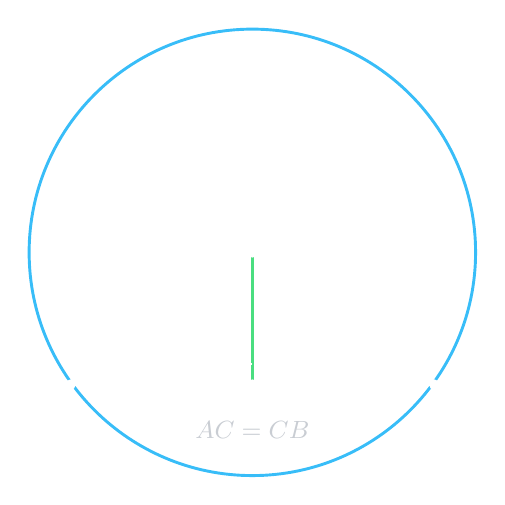
\begin{tikzpicture}[scale=1.05]
  \coordinate (O) at (0,1.6);
  \coordinate (C) at (0,0);
  \coordinate (A) at (-2.2,0);
  \coordinate (B) at (2.2,0);

  \draw[cline] (O) circle (2.7);
  \draw[line] (A)--(B);
  \draw[gline] (O)--(C);
  \draw[line] (-0.25,0) -- (-0.25,0.25) -- (0,0.25);

  \fill (O) node[dot]{} node[lbl, right] {$O$};
  \fill (C) node[dot]{} node[lbl, below] {$C$};
  \fill (A) node[dot]{} node[lbl, below left] {$A$};
  \fill (B) node[dot]{} node[lbl, below right] {$B$};

  \node[mlabel] at (0,-0.55) {$AC=CB$};
\end{tikzpicture}
}

\Step{3.} In right $\triangle OCA$:
\[
OA^2=OC^2+AC^2
\Rightarrow 13^2=5^2+AC^2
\Rightarrow AC=12\text{ cm}.
\]
\StepFig{Step 3 diagram (right triangle $OCA$)}{%
\begin{tikzpicture}[scale=1.05]
  \coordinate (C) at (0,0);
  \coordinate (A) at (-2.6,0);
  \coordinate (O) at (0,2.0);

  \draw[line] (A)--(C)--(O)--cycle;
  \draw[line] (-0.25,0) -- (-0.25,0.25) -- (0,0.25);

  \fill (O) node[dot]{} node[lbl, right] {$O$};
  \fill (C) node[dot]{} node[lbl, below] {$C$};
  \fill (A) node[dot]{} node[lbl, below left] {$A$};

  \node[lbl] at (-1.3,-0.35) {$AC$};
  \node[lbl] at (0.55,1.1) {$OC=5$};
  \node[lbl] at (-1.25,1.15) {$OA=13$};
\end{tikzpicture}
}

\Step{4.} Therefore:
\[
AB=2AC=24\text{ cm}.
\]
\StepFig{Step 4 diagram (double the half-chord)}{%
\begin{tikzpicture}[scale=1.05]
  \coordinate (C) at (0,0);
  \coordinate (A) at (-2.8,0);
  \coordinate (B) at (2.8,0);

  \draw[line] (A)--(B);
  \fill (C) node[dot]{} node[lbl, below] {$C$};
  \fill (A) node[dot]{} node[lbl, below left] {$A$};
  \fill (B) node[dot]{} node[lbl, below right] {$B$};

  \node[lbl] at (-1.4,-0.35) {$12$};
  \node[lbl] at (1.4,-0.35) {$12$};
  \node[mlabel] at (0,-0.85) {$AB=24$};
\end{tikzpicture}
}
\end{QAPair}

% ============================================================
% Q6
\begin{QAPair}{Question 6}
\textcolor{gold}{\bfseries Question:}
Construct a rectangle $EFGH$ such that $EF=6$ cm and $FG=4$ cm. Draw a circle passing through its vertices and prove that it is the only circle that can be drawn through the vertices.\\
\tcblower
\textcolor{green}{\bfseries Answer:}

\Step{1 (Draw $EF=6$ cm).}
\StepFig{Step 1 diagram}{%
\begin{tikzpicture}[scale=1.0]
  \coordinate (E) at (0,0);
  \coordinate (F) at (6,0);
  \draw[line] (E)--(F);
  \fill (E) node[dot]{} node[lbl, below left] {$E$};
  \fill (F) node[dot]{} node[lbl, below right] {$F$};
  \node[lbl] at (3,-0.55) {$6\text{ cm}$};
\end{tikzpicture}
}

\Step{2 (At $F$, draw a perpendicular and mark $FG=4$ cm).}
\StepFig{Step 2 diagram}{%
\begin{tikzpicture}[scale=1.0]
  \coordinate (E) at (0,0);
  \coordinate (F) at (6,0);
  \coordinate (G) at (6,4);

  \draw[line] (E)--(F);
  \draw[line] (F)--(G);

  \draw[line] (5.75,0) -- (5.75,0.25) -- (6,0.25);

  \fill (E) node[dot]{} node[lbl, below left] {$E$};
  \fill (F) node[dot]{} node[lbl, below right] {$F$};
  \fill (G) node[dot]{} node[lbl, right] {$G$};

  \node[lbl] at (6.55,2) {$4\text{ cm}$};
\end{tikzpicture}
}

\Step{3 (Complete rectangle by drawing parallels to meet at $H$).}
\StepFig{Step 3 diagram}{%
\begin{tikzpicture}[scale=1.0]
  \coordinate (E) at (0,0);
  \coordinate (F) at (6,0);
  \coordinate (G) at (6,4);
  \coordinate (H) at (0,4);

  \draw[line] (E)--(F)--(G)--(H)--cycle;

  \fill (E) node[dot]{} node[lbl, below left] {$E$};
  \fill (F) node[dot]{} node[lbl, below right] {$F$};
  \fill (G) node[dot]{} node[lbl, above right] {$G$};
  \fill (H) node[dot]{} node[lbl, above left] {$H$};

  \node[mlabel] at (3,-0.55) {$EF=6$};
  \node[mlabel] at (6.55,2) {$FG=4$};
\end{tikzpicture}
}

\Step{4 (Draw diagonals; they meet at $O$).}
\StepFig{Step 4 diagram}{%
\begin{tikzpicture}[scale=1.0]
  \coordinate (E) at (0,0);
  \coordinate (F) at (6,0);
  \coordinate (G) at (6,4);
  \coordinate (H) at (0,4);
  \coordinate (O) at (3,2);

  \draw[line] (E)--(F)--(G)--(H)--cycle;
  \draw[dashedline] (E)--(G);
  \draw[dashedline] (F)--(H);

  \fill (O) node[dot]{} node[lbl, right] {$O$};
  \fill (E) node[dot]{} node[lbl, below left] {$E$};
  \fill (F) node[dot]{} node[lbl, below right] {$F$};
  \fill (G) node[dot]{} node[lbl, above right] {$G$};
  \fill (H) node[dot]{} node[lbl, above left] {$H$};
\end{tikzpicture}
}

\Step{5 (Draw circle with centre $O$ and radius $OE$).}
\StepFig{Step 5 diagram (circle through all four vertices)}{%
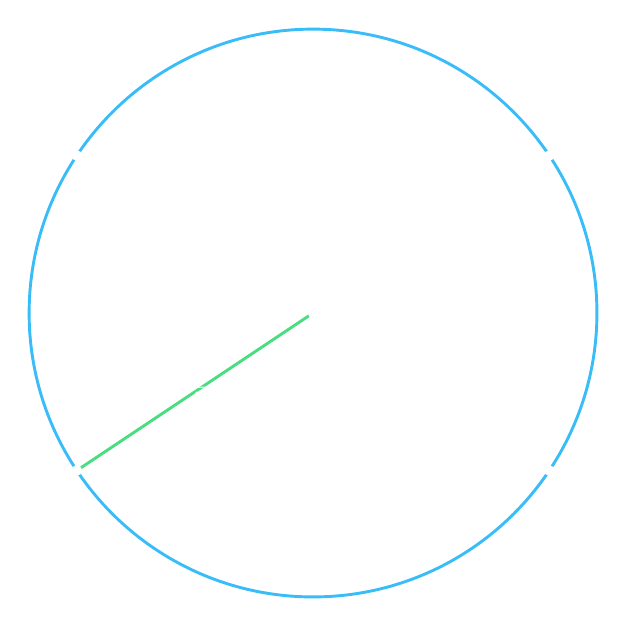
\begin{tikzpicture}[scale=1.0]
  \coordinate (E) at (0,0);
  \coordinate (F) at (6,0);
  \coordinate (G) at (6,4);
  \coordinate (H) at (0,4);
  \coordinate (O) at (3,2);

  \draw[cline] (O) circle ({0.5*sqrt(6^2+4^2)});
  \draw[line] (E)--(F)--(G)--(H)--cycle;
  \draw[gline] (O)--(E);

  \fill (O) node[dot]{} node[lbl, right] {$O$};
  \fill (E) node[dot]{} node[lbl, below left] {$E$};
  \fill (F) node[dot]{} node[lbl, below right] {$F$};
  \fill (G) node[dot]{} node[lbl, above right] {$G$};
  \fill (H) node[dot]{} node[lbl, above left] {$H$};

  \node[lbl] at (1.75,1.05) {$R=OE$};
\end{tikzpicture}
}

\Step{6 (Uniqueness).}
A circle through three non-collinear points is unique.
Since $E,F,G$ are non-collinear, only one circle passes through $E,F,G$.
Our construction gives a circle through $E,F,G$ and also through $H$, hence it is the \emph{only} circle through all four vertices.

\StepFig{Step 6 diagram (3 points fix one circle)}{%
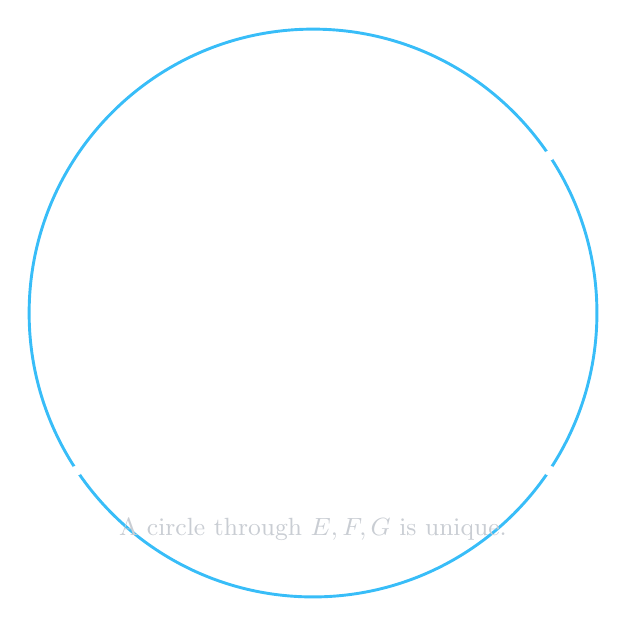
\begin{tikzpicture}[scale=1.0]
  \coordinate (E) at (0,0);
  \coordinate (F) at (6,0);
  \coordinate (G) at (6,4);
  \coordinate (O) at (3,2);

  \draw[cline] (O) circle ({0.5*sqrt(6^2+4^2)});
  \fill (E) node[dot]{} node[lbl, below left] {$E$};
  \fill (F) node[dot]{} node[lbl, below right] {$F$};
  \fill (G) node[dot]{} node[lbl, above right] {$G$};

  \node[mlabel] at (3,-0.75) {A circle through $E,F,G$ is unique.};
\end{tikzpicture}
}
\end{QAPair}

% ============================================================
% Q7
\begin{QAPair}{Question 7}
\textcolor{gold}{\bfseries Question:}
Take four non-collinear points $A,B,C,D$ such that $AB=BC=DB=4$ cm.
Draw all possible circles that can pass through $A, C$ and $D$.\\
\tcblower
\textcolor{green}{\bfseries Answer:}

\Step{1.} $AB=BC=BD=4$ cm $\Rightarrow$ $B$ is equidistant from $A,C,D$.

\StepFig{Step 1 diagram (equal radii from $B$)}{%
\begin{tikzpicture}[scale=1.0]
  \coordinate (B) at (0,0);
  \coordinate (A) at (-2.8,0.4);
  \coordinate (C) at (1.6,2.4);
  \coordinate (D) at (2.6,-1.3);

  \draw[gline] (B)--(A);
  \draw[gline] (B)--(C);
  \draw[gline] (B)--(D);

  \fill (A) node[dot]{} node[lbl, left] {$A$};
  \fill (B) node[dot]{} node[lbl, below] {$B$};
  \fill (C) node[dot]{} node[lbl, above] {$C$};
  \fill (D) node[dot]{} node[lbl, right] {$D$};

  \node[mlabel] at (0.15,1.15) {$BA=BC=BD$};
\end{tikzpicture}
}

\Step{2.} So $B$ is the circumcentre of $\triangle ACD$.

\StepFig{Step 2 diagram (circumcentre at $B$)}{%
\begin{tikzpicture}[scale=1.0]
  \coordinate (B) at (0,0);
  \coordinate (A) at (-2.8,0.4);
  \coordinate (C) at (1.6,2.4);
  \coordinate (D) at (2.6,-1.3);

  \draw[line] (A)--(C)--(D)--cycle;
  \fill (B) node[dot]{} node[lbl, below] {$B$};

  \node[mlabel] at (-0.1,-1.9) {$B$ is equidistant from $A,C,D$.};
\end{tikzpicture}
}

\Step{3.} Hence the circle through $A,C,D$ is the circle with centre $B$ and radius $4$ cm, and it is unique.

\StepFig{Step 3 diagram (the only circle)}{%
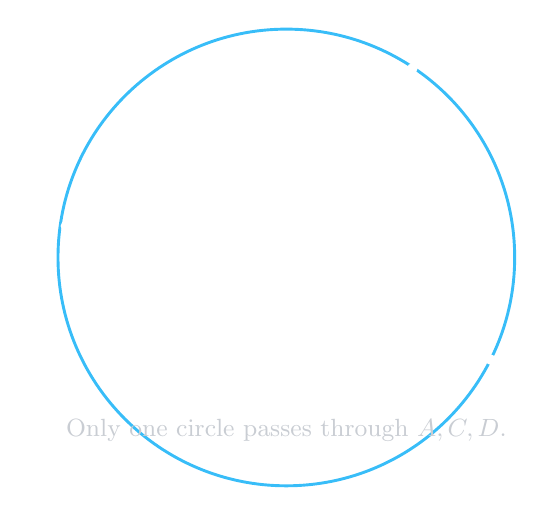
\begin{tikzpicture}[scale=1.0]
  \coordinate (B) at (0,0);
  \coordinate (A) at (-2.8,0.4);
  \coordinate (C) at (1.6,2.4);
  \coordinate (D) at (2.6,-1.3);

  \draw[cline] (B) circle (2.9);
  \fill (A) node[dot]{} node[lbl, left] {$A$};
  \fill (B) node[dot]{} node[lbl, below] {$B$};
  \fill (C) node[dot]{} node[lbl, above] {$C$};
  \fill (D) node[dot]{} node[lbl, right] {$D$};

  \node[mlabel] at (0,-2.2) {Only one circle passes through $A,C,D$.};
\end{tikzpicture}
}
\end{QAPair}

% ============================================================
% Q8(i)
\begin{QAPair}{Question 8 (i)}
\textcolor{gold}{\bfseries Question:}
In the diagram, $PU=16$ cm and $RS=10$ cm. Express $OU$ in terms of radius $r$.
(Hint: $16-OU=r$.)\\
\tcblower
\textcolor{green}{\bfseries Answer:}

\Step{1.} Along the diameter, $PU=PO+OU$ and $PO=r$:
\[
16=r+OU \quad\Rightarrow\quad OU=16-r.
\]

\StepFig{Step 1 diagram (diameter segment split)}{%
\begin{tikzpicture}[scale=1.05]
  \coordinate (P) at (0,0);
  \coordinate (U) at (3.0,0);
  \coordinate (O) at (1.3,0);

  \draw[line] (P)--(U);
  \fill (P) node[dot]{} node[lbl, below] {$P$};
  \fill (O) node[dot]{} node[lbl, below] {$O$};
  \fill (U) node[dot]{} node[lbl, below] {$U$};

  \node[lbl] at (0.65,0.35) {$PO=r$};
  \node[lbl] at (2.15,0.35) {$OU$};
  \node[mlabel] at (1.5,-0.65) {$PU=16$};
\end{tikzpicture}
}
\end{QAPair}

% ============================================================
% Q8(ii)
\begin{QAPair}{Question 8 (ii)}
\textcolor{gold}{\bfseries Question:}
Form an equation in $r$ and solve it to find the radius $r$.\\
\tcblower
\textcolor{green}{\bfseries Answer:}

\Step{1.} $OU\perp RS$ $\Rightarrow$ $U$ bisects chord $RS$:
\[
UR=\frac{RS}{2}=\frac{10}{2}=5\text{ cm}.
\]
\StepFig{Step 1 diagram (bisected chord)}{%
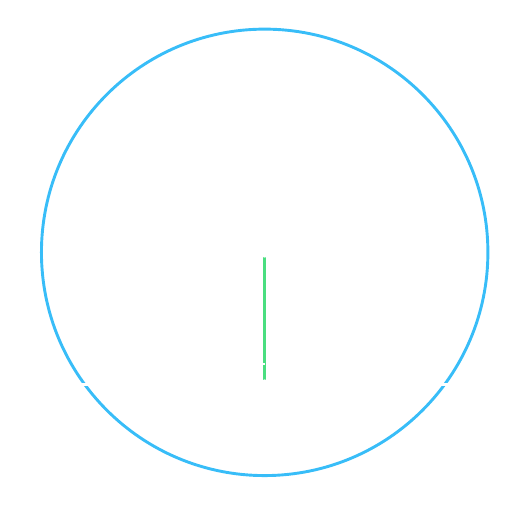
\begin{tikzpicture}[scale=1.05]
  \coordinate (O) at (0,1.6);
  \coordinate (U) at (0,0);
  \coordinate (R) at (-2.4,0);
  \coordinate (S) at (2.4,0);

  \draw[cline] (O) circle (2.7);
  \draw[line] (R)--(S);
  \draw[gline] (O)--(U);
  \draw[line] (-0.25,0) -- (-0.25,0.25) -- (0,0.25);

  \fill (O) node[dot]{} node[lbl, right] {$O$};
  \fill (U) node[dot]{} node[lbl, below] {$U$};
  \fill (R) node[dot]{} node[lbl, below left] {$R$};
  \fill (S) node[dot]{} node[lbl, below right] {$S$};

  \node[lbl] at (-1.2,-0.35) {$5$};
  \node[lbl] at (1.2,-0.35) {$5$};
\end{tikzpicture}
}

\Step{2.} In right $\triangle OUR$:
\[
r^2=OU^2+UR^2=OU^2+25.
\]
\StepFig{Step 2 diagram (right triangle $OUR$)}{%
\begin{tikzpicture}[scale=1.05]
  \coordinate (U) at (0,0);
  \coordinate (R) at (-2.6,0);
  \coordinate (O) at (0,2.0);

  \draw[line] (R)--(U)--(O)--cycle;
  \draw[line] (-0.25,0) -- (-0.25,0.25) -- (0,0.25);

  \fill (O) node[dot]{} node[lbl, right] {$O$};
  \fill (U) node[dot]{} node[lbl, below] {$U$};
  \fill (R) node[dot]{} node[lbl, below left] {$R$};

  \node[lbl] at (-1.3,-0.35) {$UR=5$};
  \node[lbl] at (0.55,1.1) {$OU$};
  \node[lbl] at (-1.25,1.15) {$OR=r$};
\end{tikzpicture}
}

\Step{3.} Use $r=16-OU$:
\[
(16-OU)^2=OU^2+25
\Rightarrow 256-32OU=25
\Rightarrow 32OU=231
\Rightarrow OU=\frac{231}{32}.
\]
\StepFig{Step 3 diagram (substitution map)}{%
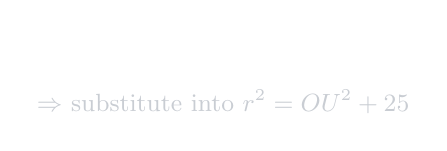
\begin{tikzpicture}[scale=1.0]
  \node[lbl, align=left] at (0,0) {$r=16-OU$};
  \node[mlabel, align=left] at (0,-0.7) {$\Rightarrow$ substitute into $r^2=OU^2+25$};
\end{tikzpicture}
}

\Step{4.} Hence:
\[
r=16-\frac{231}{32}=\frac{281}{32}\text{ cm}\approx 8.78\text{ cm}.
\]
\StepFig{Step 4 diagram (final)}{%
\begin{tikzpicture}[scale=1.0]
  \node[lbl] at (0,0) {$r=\dfrac{281}{32}\ \text{cm}\approx 8.78\ \text{cm}$};
\end{tikzpicture}
}
\end{QAPair}

% ============================================================
% Q9
\begin{QAPair}{Question 9}
\textcolor{gold}{\bfseries Question:}
In the diagram, $AB=16$ cm and $DE=4$ cm. Find the radius of the circle.\\
\tcblower
\textcolor{green}{\bfseries Answer:}

\Step{1.} Diameter $\perp$ chord $\Rightarrow$ it bisects chord:
\[
AE=EB=\frac{16}{2}=8\text{ cm}.
\]
\StepFig{Step 1 diagram (half-chord)}{%
\begin{tikzpicture}[scale=1.05]
  \coordinate (E) at (0,0);
  \coordinate (A) at (-2.8,0);
  \coordinate (B) at (2.8,0);

  \draw[line] (A)--(B);
  \fill (E) node[dot]{} node[lbl, below] {$E$};
  \fill (A) node[dot]{} node[lbl, below left] {$A$};
  \fill (B) node[dot]{} node[lbl, below right] {$B$};

  \node[lbl] at (-1.4,-0.35) {$8$};
  \node[lbl] at (1.4,-0.35) {$8$};
\end{tikzpicture}
}

\Step{2.} Let radius $r=PD$. Since $DE=4$:
\[
PE=r-4.
\]
\StepFig{Step 2 diagram (radius minus segment)}{%
\begin{tikzpicture}[scale=1.05]
  \coordinate (P) at (0,0);
  \coordinate (D) at (2.6,0);
  \coordinate (E) at (1.8,0);

  \draw[gline] (P)--(D);
  \fill (P) node[dot]{} node[lbl, below] {$P$};
  \fill (E) node[dot]{} node[lbl, below] {$E$};
  \fill (D) node[dot]{} node[lbl, below] {$D$};

  \node[lbl] at (1.3,0.35) {$PE$};
  \node[lbl] at (2.2,0.35) {$ED=4$};
  \node[mlabel] at (1.3,-0.65) {$PD=r$};
\end{tikzpicture}
}

\Step{3.} In right $\triangle PEA$:
\[
r^2=(r-4)^2+8^2
\Rightarrow r^2=r^2-8r+16+64
\Rightarrow 8r=80
\Rightarrow r=10\text{ cm}.
\]
\StepFig{Step 3 diagram (right triangle used)}{%
\begin{tikzpicture}[scale=1.05]
  \coordinate (E) at (0,0);
  \coordinate (A) at (-2.6,0);
  \coordinate (P) at (0,2.0);

  \draw[line] (A)--(E)--(P)--cycle;
  \draw[line] (-0.25,0) -- (-0.25,0.25) -- (0,0.25);

  \fill (P) node[dot]{} node[lbl, right] {$P$};
  \fill (E) node[dot]{} node[lbl, below] {$E$};
  \fill (A) node[dot]{} node[lbl, below left] {$A$};

  \node[lbl] at (-1.3,-0.35) {$AE=8$};
  \node[lbl] at (0.65,1.1) {$PE=r-4$};
  \node[lbl] at (-1.25,1.15) {$PA=r$};
\end{tikzpicture}
}
\end{QAPair}

% ============================================================
% Q10
\begin{QAPair}{Question 10}
\textcolor{gold}{\bfseries Question:}
Given that diameter and chord of a circle are $10$ cm and $8$ cm long respectively.
The diameter bisects the chord and the distance between chord and centre of the circle is $3$ cm.
Show that the diameter bisects the chord perpendicularly.\\
\tcblower
\textcolor{green}{\bfseries Answer:}

\Step{1 (Label the figure).}
Let $O$ be the centre, $AB$ be the chord with $AB=8$ cm, and the diameter meet $AB$ at $M$.
Given the diameter bisects the chord:
\[
AM=MB=\frac{8}{2}=4\text{ cm}.
\]

\StepFig{Step 1 diagram (label chord + midpoint)}{%
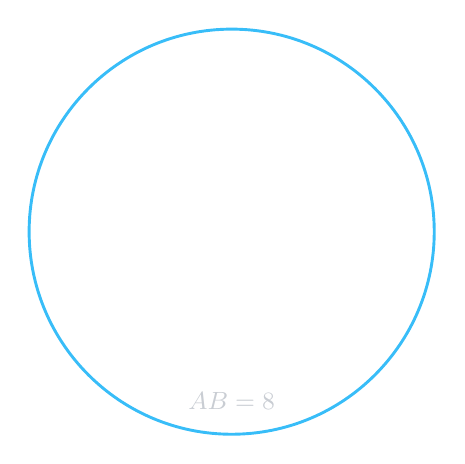
\begin{tikzpicture}[scale=1.05]
  \coordinate (O) at (0,0.7);
  \def\r{2.45}
  \draw[cline] (O) circle (\r);

  \coordinate (M) at (0,-0.55);
  \coordinate (A) at (-2.0,-0.55);
  \coordinate (B) at ( 2.0,-0.55);

  \draw[line] (A)--(B);
  \fill (O) node[dot]{} node[lbl, above right]{$O$};
  \fill (M) node[dot]{} node[lbl, below]{$M$};
  \fill (A) node[dot]{} node[lbl, below left]{$A$};
  \fill (B) node[dot]{} node[lbl, below right]{$B$};

  \node[lbl] at (-1.0,-0.95) {$4$};
  \node[lbl] at ( 1.0,-0.95) {$4$};
  \node[mlabel] at (0,-1.35) {$AB=8$};
\end{tikzpicture}
}

\Step{2 (Use radii).}
Diameter is $10$ cm, so radius:
\[
OA=OB=5\text{ cm}.
\]
Also the distance from centre to chord is:
\[
OM=3\text{ cm}.
\]

\StepFig{Step 2 diagram (show $OA=5$ and $OM=3$)}{%
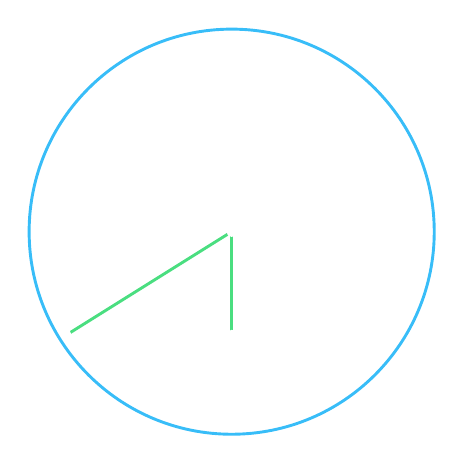
\begin{tikzpicture}[scale=1.05]
  \coordinate (O) at (0,0.7);
  \def\r{2.45}
  \draw[cline] (O) circle (\r);

  \coordinate (M) at (0,-0.55);
  \coordinate (A) at (-2.0,-0.55);

  \draw[gline] (O)--(M);
  \draw[gline] (O)--(A);

  \fill (O) node[dot]{} node[lbl, above right]{$O$};
  \fill (M) node[dot]{} node[lbl, below]{$M$};
  \fill (A) node[dot]{} node[lbl, below left]{$A$};

  \node[lbl] at (-1.05,0.55) {$OA=5$};
  \node[lbl] at (0.75,0.15) {$OM=3$};
\end{tikzpicture}
}

\Step{3 (Congruent triangles).}
Consider triangles $\triangle OMA$ and $\triangle OMB$:
\[
OA=OB \ (\text{radii}),\quad
OM=OM \ (\text{common}),\quad
AM=MB \ (\text{given}).
\]
Therefore,
\[
\triangle OMA \cong \triangle OMB \quad (\text{SSS}).
\]

\StepFig{Step 3 diagram (two triangles share $OM$)}{%
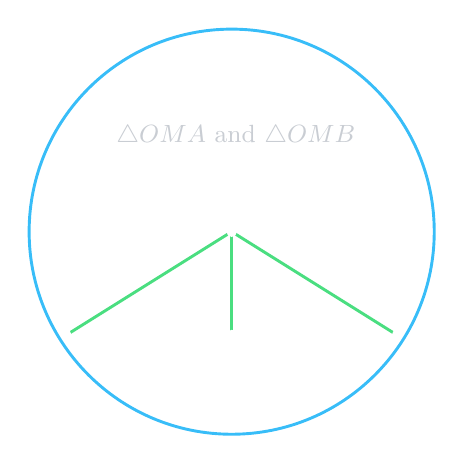
\begin{tikzpicture}[scale=1.05]
  \coordinate (O) at (0,0.7);
  \def\r{2.45}
  \draw[cline] (O) circle (\r);

  \coordinate (M) at (0,-0.55);
  \coordinate (A) at (-2.0,-0.55);
  \coordinate (B) at ( 2.0,-0.55);

  \draw[line] (A)--(B);
  \draw[gline] (O)--(M);
  \draw[gline] (O)--(A);
  \draw[gline] (O)--(B);

  \fill (O) node[dot]{} node[lbl, above right]{$O$};
  \fill (M) node[dot]{} node[lbl, below]{$M$};
  \fill (A) node[dot]{} node[lbl, below left]{$A$};
  \fill (B) node[dot]{} node[lbl, below right]{$B$};

  \node[mlabel] at (0.05,1.85) {$\triangle OMA$ and $\triangle OMB$};
\end{tikzpicture}
}

\Step{4 (Right angle at the chord).}
So corresponding angles are equal:
\[
\angle OMA=\angle OMB.
\]
But $A,M,B$ are collinear, hence
\[
\angle OMA+\angle OMB=180^\circ.
\]
Equal angles summing to $180^\circ$ must each be $90^\circ$, so
\[
\angle OMA=\angle OMB=90^\circ \Rightarrow OM\perp AB.
\]
Thus the diameter bisects the chord \emph{perpendicularly}.

\StepFig{Step 4 diagram (perpendicular shown)}{%
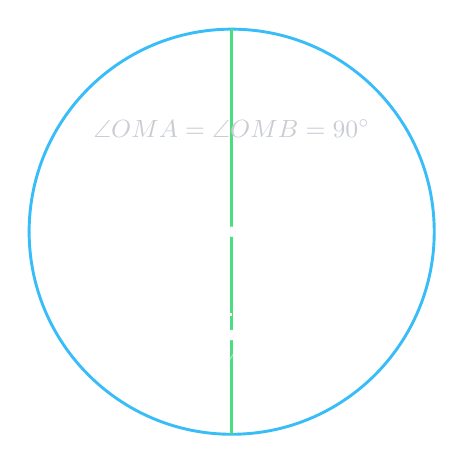
\begin{tikzpicture}[scale=1.05]
  \coordinate (O) at (0,0.7);
  \def\r{2.45}
  \draw[cline] (O) circle (\r);

  \coordinate (M) at (0,-0.55);
  \coordinate (A) at (-2.0,-0.55);
  \coordinate (B) at ( 2.0,-0.55);

  \coordinate (Top) at (0,{0.7+\r});
  \coordinate (Bot) at (0,{0.7-\r});

  \draw[line] (A)--(B);
  \draw[gline] (Top)--(Bot);

  \draw[line] (-0.25,-0.55) -- (-0.25,-0.30) -- (0,-0.30);

  \fill (O) node[dot]{} node[lbl, above right]{$O$};
  \fill (M) node[dot]{} node[lbl, below]{$M$};
  \fill (A) node[dot]{} node[lbl, below left]{$A$};
  \fill (B) node[dot]{} node[lbl, below right]{$B$};

  \node[mlabel] at (0,1.95) {$\angle OMA=\angle OMB=90^\circ$};
\end{tikzpicture}
}
\end{QAPair}

% ============================================================
% Q11
\begin{QAPair}{Question 11}
\textcolor{gold}{\bfseries Question:}
In the figure $O$ is centre of the circle. $AB$ is the chord and $CD \perp AB$ passes through centre.
Show that $AC = BC$.\\
\tcblower
\textcolor{green}{\bfseries Answer:}

\Step{1 (Use the centre-perpendicular fact).}
Since $O$ is the centre and $CD\perp AB$ passes through $O$, the perpendicular from the centre to a chord bisects the chord.
So if $D$ is the foot on $AB$, then
\[
AD=DB.
\]

\StepFig{Step 1 diagram (centre $\perp$ chord bisects chord)}{%
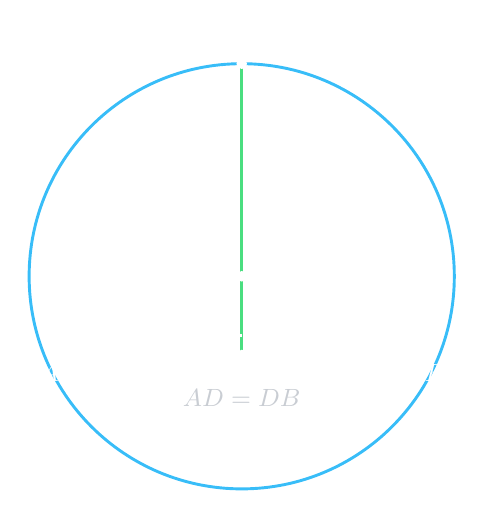
\begin{tikzpicture}[scale=1.0]
  \coordinate (O) at (0,0);
  \draw[cline] (O) circle (2.7);

  \coordinate (C) at (0,2.7);
  \coordinate (D) at (0,-1.0);
  \coordinate (A) at (-2.2,-1.0);
  \coordinate (B) at (2.2,-1.0);

  \draw[line] (A)--(B);
  \draw[gline] (C)--(D);

  \draw[line] (-0.25,-1.0) -- (-0.25,-0.75) -- (0,-0.75);

  \fill (O) node[dot] {} node[lbl, left] {$O$};
  \fill (C) node[dot] {} node[lbl, above] {$C$};
  \fill (D) node[dot] {} node[lbl, below] {$D$};
  \fill (A) node[dot] {} node[lbl, below left] {$A$};
  \fill (B) node[dot] {} node[lbl, below right] {$B$};

  \node[mlabel] at (0,-1.55) {$AD=DB$};
\end{tikzpicture}
}

\Step{2 (Identify right triangles).}
Triangles $\triangle ADC$ and $\triangle BDC$ are right triangles (right angle at $D$), and they share side $CD$:
\[
\angle ADC=\angle BDC=90^\circ,\qquad CD=CD.
\]

\StepFig{Step 2 diagram (two right triangles)}{%
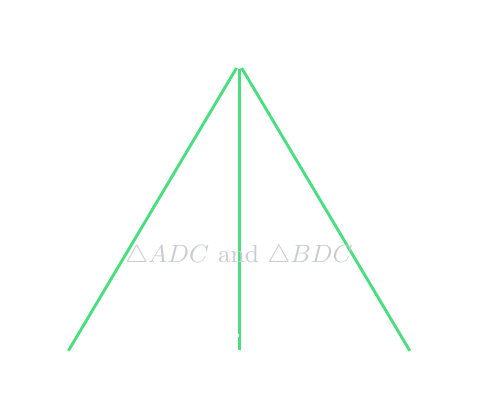
\begin{tikzpicture}[scale=1.0]
  \coordinate (C) at (0,2.7);
  \coordinate (D) at (0,-1.0);
  \coordinate (A) at (-2.2,-1.0);
  \coordinate (B) at (2.2,-1.0);

  \draw[line] (A)--(B);
  \draw[gline] (C)--(D);
  \draw[gline] (C)--(A);
  \draw[gline] (C)--(B);

  \draw[line] (-0.25,-1.0) -- (-0.25,-0.75) -- (0,-0.75);

  \fill (C) node[dot] {} node[lbl, above] {$C$};
  \fill (D) node[dot] {} node[lbl, below] {$D$};
  \fill (A) node[dot] {} node[lbl, below left] {$A$};
  \fill (B) node[dot] {} node[lbl, below right] {$B$};

  \node[mlabel] at (0,0.25) {$\triangle ADC$ and $\triangle BDC$};
\end{tikzpicture}
}

\Step{3 (Apply congruence).}
From Step 1, $AD=DB$. Also $CD$ is common and both triangles are right-angled at $D$.
So
\[
\triangle ADC \cong \triangle BDC \quad (\text{RHS}).
\]

\StepFig{Step 3 diagram (matching parts)}{%
\begin{tikzpicture}[scale=1.0]
  \coordinate (C) at (0,2.7);
  \coordinate (D) at (0,-1.0);
  \coordinate (A) at (-2.2,-1.0);
  \coordinate (B) at (2.2,-1.0);

  \draw[gline] (C)--(D);
  \draw[line] (A)--(D);
  \draw[line] (D)--(B);
  \draw[line] (C)--(A);
  \draw[line] (C)--(B);

  \fill (C) node[dot] {} node[lbl, above] {$C$};
  \fill (D) node[dot] {} node[lbl, below] {$D$};
  \fill (A) node[dot] {} node[lbl, below left] {$A$};
  \fill (B) node[dot] {} node[lbl, below right] {$B$};

  \node[mlabel] at (0,-1.75) {$AD=DB$ and $CD$ common};
\end{tikzpicture}
}

\Step{4 (Conclude).}
Therefore corresponding hypotenuses are equal:
\[
AC=BC.
\]

\StepFig{Step 4 diagram (result highlighted)}{%
\begin{tikzpicture}[scale=1.0]
  \coordinate (C) at (0,2.7);
  \coordinate (A) at (-2.2,-1.0);
  \coordinate (B) at (2.2,-1.0);

  \draw[gline] (C)--(A);
  \draw[gline] (C)--(B);

  \fill (C) node[dot] {} node[lbl, above] {$C$};
  \fill (A) node[dot] {} node[lbl, below left] {$A$};
  \fill (B) node[dot] {} node[lbl, below right] {$B$};

  \node[lbl] at (-0.95,1.0) {$AC$};
  \node[lbl] at (0.95,1.0) {$BC$};
  \node[mlabel] at (0,-1.75) {$AC=BC$};
\end{tikzpicture}
}
\end{QAPair}

\end{document}
